\section{Theoretical background}

\subsection{Markov Decision Processes}

Markov Decision Processes (MDPs) are a classical formalization of sequential decision making, where actions influence not just immediate rewards, but also subsequent situations (states) and through those future rewards. Thus MDPs involve delayed reward and the need to tradeoff immediate and delayed reward.

A Markov Decision Process consists of a set of states $S$ and a set of actions $A$. The dynamics of the MDP, from any state $s \in S$ and for any action $a \in A$, are determined by transition probabilities, $P^a_{ss'} = Pr(s_{t+1} = s' | s_t = s, a_t = a)$, specifying the distribution over the next state $s' \in S$. Finally, a reward function, $R^a_{ss'} = \EX[r_{t+1} | s_t = s, a_t = a, s_{t+1} = s']$, specifies the expected reward for a given state transition.
Episodic MDPs terminate with probability 1 in a distinguished terminal state, $s_T \in S$, after finite number of transitions. Continuous MDPs does not include the terminal state and can run endlessly.
The return $R_t = \sum^T_{k=t}r_k$ is the total reward accumulated in that episode from time $t$ until reaching the terminal state at time $T$. In continuous MDPs this is the sum of an infinite sequence of rewards from time $t$.
A policy, $\pi(s, a) = Pr(a_t = a | s_t = s)$, maps a state $s$ to a probability distribution over actions.
The value function, $V_\pi(s) = \EX_\pi[R_t | s_t = s]$, is the expected return from state $s$ when following policy $\pi$.
The action value function, $Q_\pi(s, a) = \EX_\pi[R_t | s_t = s, a_t = a]$, is the expected return after selecting action $a$ in state $s$ and then following policy $\pi$.
The optimal value function is the unique value function that maximises the value of every state, $V^*(s) = maxV_\pi(s), \forall_{s \in S}$ and $Q^*(s, a) = maxQ_\pi(s, a), \forall_{s \in S, a \in A}$. An optimal policy $\pi^*(s, a)$ is a policy that maximises the action value function from every state in the MDP, $\pi^*(s, a) = \underset{a}{\mathrm{argmax}}Q^*(s, a)$.

MDPs are a mathematically idealized form of the reinforcement learning problem for which precise theoretical statements can be made. In reinforcement learning the dynamics and the reward function are hidden behind an environment. Consequently, we can not directly use them for planning, but we can learn through interaction with the environment.

\subsection{Reinforcement Learning}

Reinforcement learning (RL) is learning what to do, how to map situations to actions, so as to maximize a numerical reward signal.\cite{Book.RLAI} This mapping is called a policy $\pi$. RL consists of an agent that, in order to learn a good policy, acts in an environment. The environment provides a response to each agent's action $a$ that is interpreted and fed back to the agent. Reward $r$ is used as a reinforcing signal and state $s$ is used to condition agent's decisions. Fig.~\ref{Fig.RL} explains it in the diagram.
Each action-response-interpretation sequence is called a step or a transition. Multiple steps form an episode. The episode finishes in a terminal state $s_T$ and the environment is reset in order to start the next episode from scratch. Very often, RL agents need dozens and dozens of episodes to gather enough experience to learn the (near) optimal policy.

\begin{figure}[H]
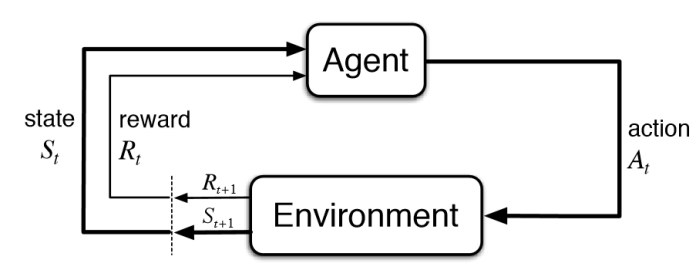
\includegraphics[]{figures/RL.jpg}
\caption[Reinforcement Learning]{Reinforcement Learning\protect\cite{Book.RLAI}}
\label{Fig.RL}
\end{figure}

\editnote{Should I describe here General Policy Iteration, Monte-Carlo Control, TD-Learning, ... what else? Rather than guessing what needs to be described, continue work and see what needs more attention.}

\subsection{Deep Learning}

Machine learning gives AI systems the ability to acquire their own knowledge, by extracting patterns from raw data. In stands in opposition to classical computer programs which execute explicit instructions hand-coded by a programmer.
One example of machine learning algorithm is logistic regression. It can determine whether to recommend cesarean delivery or not\cite{Study.Cesarean}. Another widely used machine learning algorithm called naive Bayes can distinguish between legitimate and spam e-mail.

The performance of these machine learning algorithms depends heavily on the representation of the problem they are given. For example, when logistic regression is used to recommend cesarean delivery, the AI system does not examine the patient's MRI scan directly. It would not be able to make useful predictions as individual pixels in an MRI scan have negligible correlation with any complications that might occur during delivery. It, instead, gets several pieces of relevant information, such as the presence or absence of a uterine scar, from the doctor. Each piece of information included in the representation of the data is known as a feature. Logistic regression learns the relation between those features and various outcomes, such as a recommendation of cesarean delivery. The algorithm does not influence the way that the features are defined in any way.

Sometimes it can be hard to hand-craft a good problem's representation. For example, suppose that we would like to write a program to detect cats in photographs. We know that cats are furry and have whiskers, so we might like to use the presence of a fur and whiskers as features. Unfortunately, it is difficult to describe exactly what a fur or a whisker looks like in terms of pixel values. This gets even more complicated when we take into account e.g. shadows falling on the cat or an object in the foreground obscuring part of the animal.
One solution to this problem is to use machine learning to discover not only the mapping from representation to output but also the representation itself. This approach is known as representation learning. Learned representations often result in much better performance of machine learning algorithms than can be obtained with hand-designed representations. They also allow AI systems to rapidly adapt to new tasks with minimal human intervention.

Deep learning is a particular kind of machine learning that achieves great power and flexibility by learning to represent the world as a nested hierarchy of concepts, with each concept defined in relation to simpler concepts. Deep learning solves representation learning problem by introducing representations that are expressed in terms of other, simpler representations. Fig.~\ref{Fig.DL} shows how a deep learning system can represent the concept of an image of a person by combining simpler concepts, such as corners and contours, which are in turn defined in terms of edges.

\begin{figure}[H]
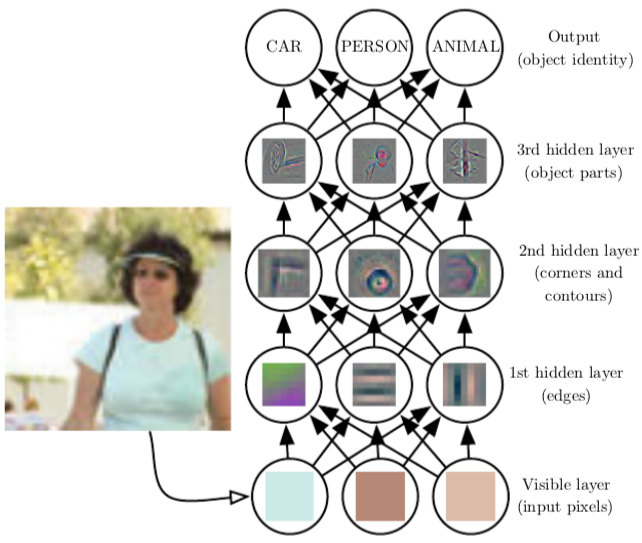
\includegraphics[width=0.8\textwidth,keepaspectratio]{figures/DL.png}
\caption[Deep Learning]{Deep Learning\protect\cite{Book.DeepLearning}}
\label{Fig.DL}
\end{figure}

The fundamental example of a deep learning model is a feedforward deep network or multilayer perceptron (MLP). A multilayer perceptron is just a mathematical function mapping some set of input values to output values. The function is formed by composing many simpler functions, called perceptrons, each providing a new representation of its input to next functions. Fig.~\ref{Fig.MLP} shows example MLP and dependencies between perceptrons. The input is presented at the input layer. Then a hidden layer (or series of them) extracts increasingly abstract features from the image. These layers are called “hidden” because their values are not given in the data. Instead, the model must determine which concepts are useful for explaining the relationships in the observed data. Finally, this description of the input in terms of the features can be used to produce the output at the output layer.

\begin{figure}[H]
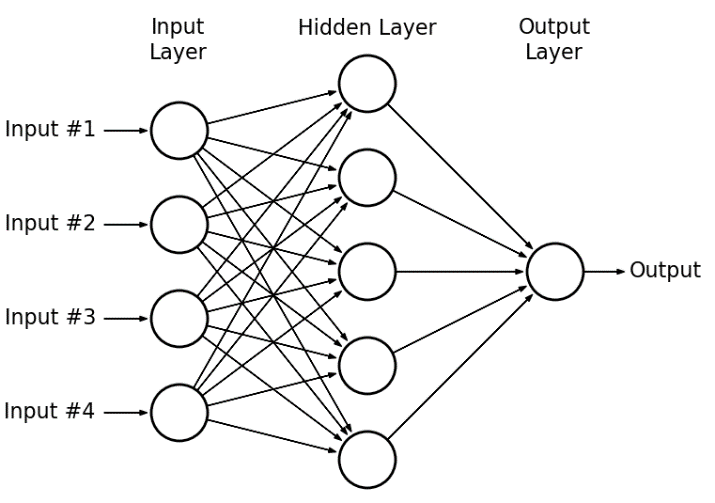
\includegraphics[width=0.8\textwidth,keepaspectratio]{figures/MLP.png}
\caption{Multilayer perceptron}
\label{Fig.MLP}
\end{figure}

\editnote{Should I mention Deep Reinforcement Learning somehow in here? Or maybe in Reinforcement Learning section?}
\editnote{Also, should I describe RNNs here if we use them later? Currently, there is citing in ``Related Work'' chapter to paper about LSTM, is it enough?}
